\documentclass[pdftex,francais]{beamer}

% Copyright 2004 by Till Tantau <tantau@users.sourceforge.net>.
%
% This file can be redistributed and/or modified under
% the terms of the GNU Public License, version 2.

%% \ifx\themename\undefined
%%   \def\themename{default}
%% \fi

\usetheme{lama}
%\usetheme{Madrid}
%\usecolortheme{crane}

\usepackage{multirow}
%\usepackage[latin1]{inputenc}           %%%  
%\usepackage[T1]{fontenc}                %%%
%\usepackage[francais]{babel}            %%%

\usepackage{multimedia}
\usepackage{hyperref}
\usepackage{tikz}
%\newtheorem{theorem}{Théorème}

%\setbeamercovered{transparent}

\title{DGtal:  Digital Geometry Tools and Algorithms}

\author[ ]{  \\[3mm]
  \small

  \normalsize
}

\date{DGCI, 2011}


\graphicspath{{Figures/},{Images/},{Graphs/}}

%%% \AtBeginSection[]
%%% {
%%%   \begin{frame}<beamer>
%%%     \frametitle{Plan}
%%%     \tableofcontents[currentsection] %,currentsubsection]
%%%   \end{frame}
%%% }


\renewcommand{\vec}[1]{\mathbf{#1}}

% space of the real numbers
\newcommand{\R}{\ensuremath{\mathbb{R}}}
% space of the integer numbers
\newcommand{\Z}{\ensuremath{\mathbb{Z}}}
% Digitization process of step h (1)
\newcommand{\Dig}[1]{\ensuremath{\mathrm{Dig}_{#1}}}
% Family of shape
\newcommand{\SF}[0]{\ensuremath{\mathbb{F}}}
% Topological boundary of X (1).
\newcommand{\TB}[1]{\ensuremath{\partial #1}}
% Discrete geometric estimator of G (1)
\newcommand{\DGE}[1]{\ensuremath{E_{#1}}}
% Reference shape of digital object O (1) with grid step $h$ (2).
\newcommand{\RS}[2]{\ensuremath{R_{#1,#2}}}

% Digital contour.
\newcommand{\DC}{\ensuremath{C}}
% Continuous contour.
\newcommand{\CC}{\ensuremath{\mathcal{C}}}
% A point indexed by i (1) on the digital contour.
\newcommand{\PT}[1]{\ensuremath{\DC_{#1}}}
% A sequence of points indexed by i (1) on the digital contour.
\newcommand{\PTS}[2]{\ensuremath{\DC_{#1,#2}}}
% Predicate stating that the digital curve is a segment between indices 1 and 2
\newcommand{\SPRED}[2]{\ensuremath{S(#1,#2)}}
% ET logique
\newcommand{\AND}[0]{\ensuremath{\wedge}}
% OU logique
\newcommand{\OR}[0]{\ensuremath{\vee}}

% Tangent direction mapping of curve C (1)
\newcommand{\TGT}[1]{\ensuremath{\theta_{#1}}}
% Integral of squared curvature of curve C (1)
\newcommand{\ISC}[1]{\ensuremath{J[#1]}}
% Smallest possible tangent direction at constraint l (1)
\newcommand{\MinTD}[1]{\ensuremath{a_{#1}}}
% Largest possible tangent direction at constraint l (1)
\newcommand{\MaxTD}[1]{\ensuremath{b_{#1}}}
% Unknown tangent direction at constraint l (1)
\newcommand{\UnkTD}[1]{\ensuremath{t_{#1}}}

% ideal multiscale criterion
\newcommand{\IMSC}[2]{\ensuremath{\mu_{#1}(#2)}}
% multiscale profile
\newcommand{\MSP}[2]{\ensuremath{\mathcal{P}_{#1}(#2)}}
% threshold flat/curve
\newcommand{\CThreshold}[0]{\ensuremath{t_{f/c}}}
% threshold noise
\newcommand{\NThreshold}[0]{\ensuremath{t_{m}}}
% noise level
\newcommand{\NL}[0]{\ensuremath{\nu}}
% slope linear regression 
\newcommand{\SLR}[2]{\ensuremath{\theta_{#1}}}





% Pencil of maximal segments around a point.
\newcommand{\PE}[1]{\ensuremath{{\mathcal P}(#1)}}
% Tangent orientation of the maximal segment.
\newcommand{\TO}[1]{\ensuremath{\theta_#1}}
% lambda function for interpolation.
\newcommand{\LF}{\ensuremath{\lambda}}
% \lambda-MS tangent orientation.
\newcommand{\LTO}[1]{\ensuremath{\hat{\theta}(#1)}}
% \lambda-MS tangent orientation variation.
\newcommand{\LTOP}[1]{\ensuremath{\hat{\theta}'(#1)}}

%\definecolor{rougeSW_}{rgb}{0.968627,0.011765,0.015686}
\definecolor{darkgreen}{rgb}{0.0,0.6,0.0}
\definecolor{lightblue}{rgb}{0.5,0.5,1.0}
\definecolor{magenta}{rgb}{1.0,0.0,1.0}
\newcommand{\alertred}[1]{{\color{red}#1}}
\newcommand{\Cb}[1]{{\color{blue}#1}}
\newcommand{\Cdg}[1]{{\color{darkgreen}#1}}
\newcommand{\textmagenta}[1]{{\color{magenta}#1}}
\newcommand{\Implies}{{\ensuremath{\Rightarrow}}}

\newcommand{\Refs}[1]{{\color{lightblue}#1}}
\newcommand{\Cite}[1]{\Refs{[#1]}}
\newcommand{\Etal}{{\em et al.}}
\newtheorem{remark}{Remarque}
% Digitization process of step h (1)
\newcommand{\DigGh}[2]{\ensuremath{\mathrm{Dig}_{#2}(#1)}}
\newcommand{\BigT}{\ensuremath{\Theta}}
\newcommand{\BigO}{\ensuremath{O}}

\newcommand{\TAN}[0]{\ensuremath{\theta}}
% Position estimator
\newcommand{\EPOS}[0]{\ensuremath{\hat{{x}}}}
% Convexity Position estimator 
\newcommand{\ECONVPOS}[0]{\ensuremath{\hat{x}^\mathrm{conv}}}
% tangent estimator base MS.
\newcommand{\ETANMS}[0]{\ensuremath{\hat{\TAN}^{\text{MS}}}}
% tangent estimator base arete du CDP.
\newcommand{\ETANEDGE}[0]{\ensuremath{\hat{\TAN}^{\text{conv}}}}
% estimateur de longueur elementaire d'un surfel (1) sur le bord discretise de X(2) de pas h(3).


\setbeamercolor{qcolor}{fg={blue!20!black},bg={blue!15!white}}
\setbeamercolor{qcoloru}{fg={blue!10!black},bg={blue!30!white}}
\newenvironment{myblock}[2]%
	       {\begin{beamerboxesrounded}[lower=qcolor,upper=qcoloru,width=#1,shadow=true]{#2}}{\end{beamerboxesrounded}}

%%%%%%%%%%%%%%%%%%%%%%%%%%%%%%%%%%%%%%%%%%%%%%%%%%%%%%%%%%%%%%%%%%%%%%%%%%%%%%%
%%%%%%%%%%%%%%%%%%%%%%%%%%%%%%%%%%%%%%%%%%%%%%%%%%%%%%%%%%%%%%%%%%%%%%%%%%%%%%%
%%%%%%%%%%%%%%%%%%%%%%%%%%%%%%%%%%%%%%%%%%%%%%%%%%%%%%%%%%%%%%%%%%%%%%%%%%%%%%%
\begin{document}

\newlength{\unquart}
\setlength{\unquart}{0.21\textwidth}

%------------------------------------------------------------------------------
\begin{frame}
  \titlepage
\end{frame}
%------------------------------------------------------------------------------

%------------------------------------------------------------------------------
\begin{frame}
  \frametitle{DGtal: topology module}
  
  \begin{block}{Objectives}
    Basic types and operations for representing a cartesian digital
    space equipped with a digital topology, and objects lying in this
    space.
  \end{block}

  \begin{itemize}
  \item Arbitrary adjacencies in $\Z^n$, but also in subdomains
  \item Digital topology = couple of adjacencies (Rosenfeld)
  \item Object = Topology + Set
  \item Operations: neighborhoods, border, connectedness and connected
    components, decomposition into digital layers, simple points
  \end{itemize}

\end{frame}
%% %------------------------------------------------------------------------------

%% %------------------------------------------------------------------------------
%% \begin{frame}
%%   \frametitle{Adjacency}

%%   \alert{Genericity} $\Rightarrow$ concept \alert{\texttt{CAdjacency}}

%%   \begin{itemize}
%%   \item Types: \texttt{Space}, \texttt{Point}, \texttt{Adjacency}
%%   \item Methods: 
%%     \begin{itemize}
%%     \item \texttt{isAdjacentTo}( p1, p2 )
%%     \item \texttt{isProperlyAdjacentTo}( p1, p2 )
%%     \item \texttt{writeNeighborhood}( p, outit )
%%     \item \texttt{writeProperNeighborhood}( p, outit )
%%     \item \texttt{writeNeighborhood}( p, outit, pred )
%%     \item \texttt{writeProperNeighborhood}( p, outit, pred )
%%     \end{itemize}
%%   \item Models: 
%%     \begin{itemize}
%%     \item \texttt{MetricAdjacency}: 4-, 8-, 6-, 18-, 26-, $2n$-, $3^n-1$- adjacencies
%%     \item \texttt{DomainAdjacency}: adjacency limited by a specified domain.
%%     \end{itemize}
%%   \end{itemize}
%% \end{frame}
%% %------------------------------------------------------------------------------

%% %------------------------------------------------------------------------------
%% \begin{frame}[fragile]
%%   \frametitle{Digital topology}
%%   \alert{Digital topology} = couple of instances of adjacencies

%%   \begin{itemize}
%%   \item template class \texttt{DigitalTopology}
%%     \scriptsize
%%     \begin{semiverbatim}
%%  typedef SpaceND< 3,int > Z3;
%%  typedef MetricAdjacency< Z3, 1 > Adj6;
%%  typedef MetricAdjacency< Z3, 2 > Adj18;
%%  typedef DigitalTopology< Adj6, Adj18 > DT6_18;

%%  Adj6 adj6;
%%  Adj18 adj18;
%%  DT6_18 dt6_18( adj6, adj18, JORDAN_DT );
%%     \end{semiverbatim}
%%     \normalsize
%%   \item Jordan topologies may be specified (for future use)
%%   \item instances are necessary (e.g., adj may not be invariant by translation)
%%   \item reverse topology is the reversed couple
%%   \end{itemize}
%% \end{frame}
%% %------------------------------------------------------------------------------

%% %------------------------------------------------------------------------------
%% \begin{frame}[fragile]
%%   \frametitle{Digital Object}

%%   \alert{Digital object} = topology $+$ digital set

%%   \begin{itemize}
%%   \item template class \texttt{Object}

%%     \scriptsize
%%     \begin{semiverbatim}
%%  typedef HyperRectDomain< Z3 > Domain; 
%%  typedef DigitalSetSelector<Domain, BIG_DS+HIGH_BEL_DS>::Type DigitalSet;
%%  typedef Object<DT6_18, DigitalSet> ObjectType;
%%  Point p1( -50, -50, -50 ); Point p2( 50, 50, 50 );
%%  Domain domain( p1, p2 );
%%  // ball of radius 30
%%  DigitalSet ball_set( domain );
%%  Shapes<Domain>::addNorm2Ball( ball_set, Point( 0, 0 ), 30 );
%%  ObjectType ball_object( dt6_18, ball_set );
%%     \end{semiverbatim}
%%     \normalsize
%%   \item Objects may be passed by value and copied without cost
%%   \item Methods:
%%     \begin{itemize}
%%     \item neighborhoods, border, geodesic neighborhoods are objects
%%     \item (lazy) connectedness, connected components
%%     \item simple points (in Z2 and Z3)
%%     \end{itemize}
%%   \end{itemize}

%% \end{frame}
%% %------------------------------------------------------------------------------

%% %------------------------------------------------------------------------------
%% \begin{frame}[fragile]
%%   \frametitle{Expander: digital layers in an object}
  
%%   \begin{itemize}
%%   \item Expansion layer by layer within an object, starting from an initial core
%%   \item core = a point or a pointset specified by iterators
%%   \item each new layer = the set of points of the object adjacent to
%%     the preceding layer
%%   \item each layer is iterable, has a digital distance to core
%%   \item finished when no more neighbor expansion is possible
%%   \item useful for \alert{connectedness}
%%   \end{itemize}
%% \end{frame}
%% %------------------------------------------------------------------------------

%% %------------------------------------------------------------------------------
%% \begin{frame}
%%   \frametitle{Expander: digital layers in an object}
%%   \begin{center}
%%     \begin{tabular}{cc}
%%       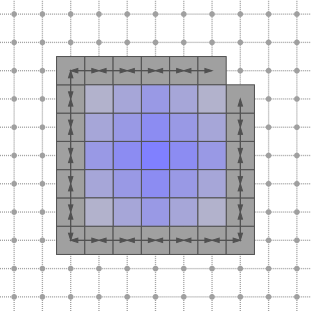
\includegraphics[width=0.4\textwidth]{house-layers4-4} &
%%       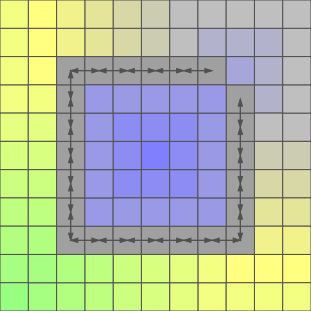
\includegraphics[width=0.4\textwidth]{house-layers4-8} \\
%%       background in 4-adj &
%%       background in 8-adj \\
%%     \end{tabular}

%%     \texttt{tests/topology/testSimpleExpander.cpp}
%%   \end{center}
%% \end{frame}

%% %------------------------------------------------------------------------------
%% \begin{frame}[fragile]
%%   \frametitle{Example: greedy homotopic thinning}
%%     \scriptsize
%%     \begin{semiverbatim}
%%   int layer = 0;
%%   do \{
%%       DigitalSet & S = shape.pointSet();
%%       std::queue<DigitalSet::Iterator> Q;
%%       for ( DigitalSet::Iterator it = S.begin(); it != S.end(); ++it )
%%         if ( shape.\alertred{isSimple}( *it ) )
%%           Q.push( it );
%%       nb_simple = 0;
%%       while ( ! Q.empty() ) \{
%%         DigitalSet::Iterator it = Q.front();
%%         Q.pop();
%%         if ( shape.isSimple( *it ) ) \{
%%           S.erase( *it );
%%           ++nb_simple;
%%         \}
%%       \}
%%       ++layer;
%%   \} while ( nb_simple != 0 );
%%     \end{semiverbatim}
%%     \normalsize
%%     See \texttt{testObject.cpp}
%% \end{frame}
%% %------------------------------------------------------------------------------

%% %------------------------------------------------------------------------------
%% \begin{frame}[fragile]
%%   \frametitle{Example: greedy homotopic thinning}
%%   \begin{center}
%%     \begin{tabular}{cc}
%%       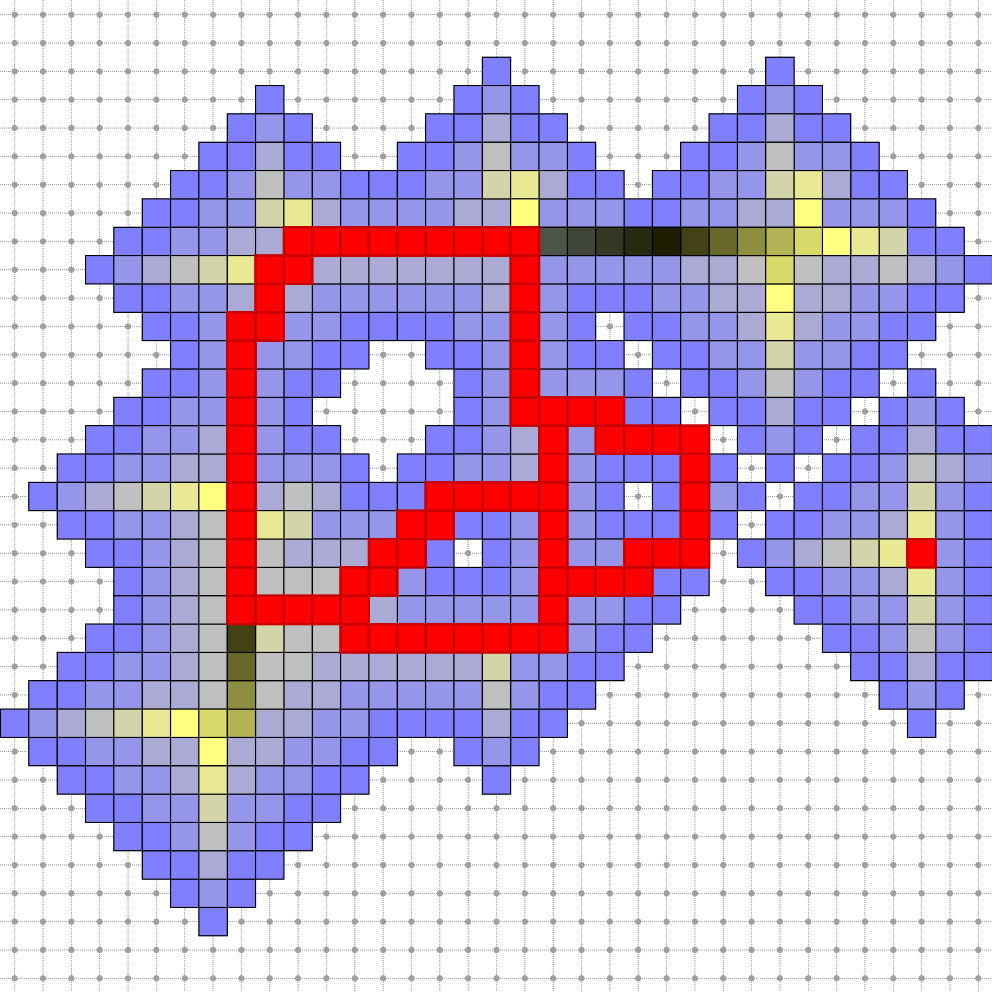
\includegraphics[width=0.4\textwidth]{shape-thinning-4-8} &
%%       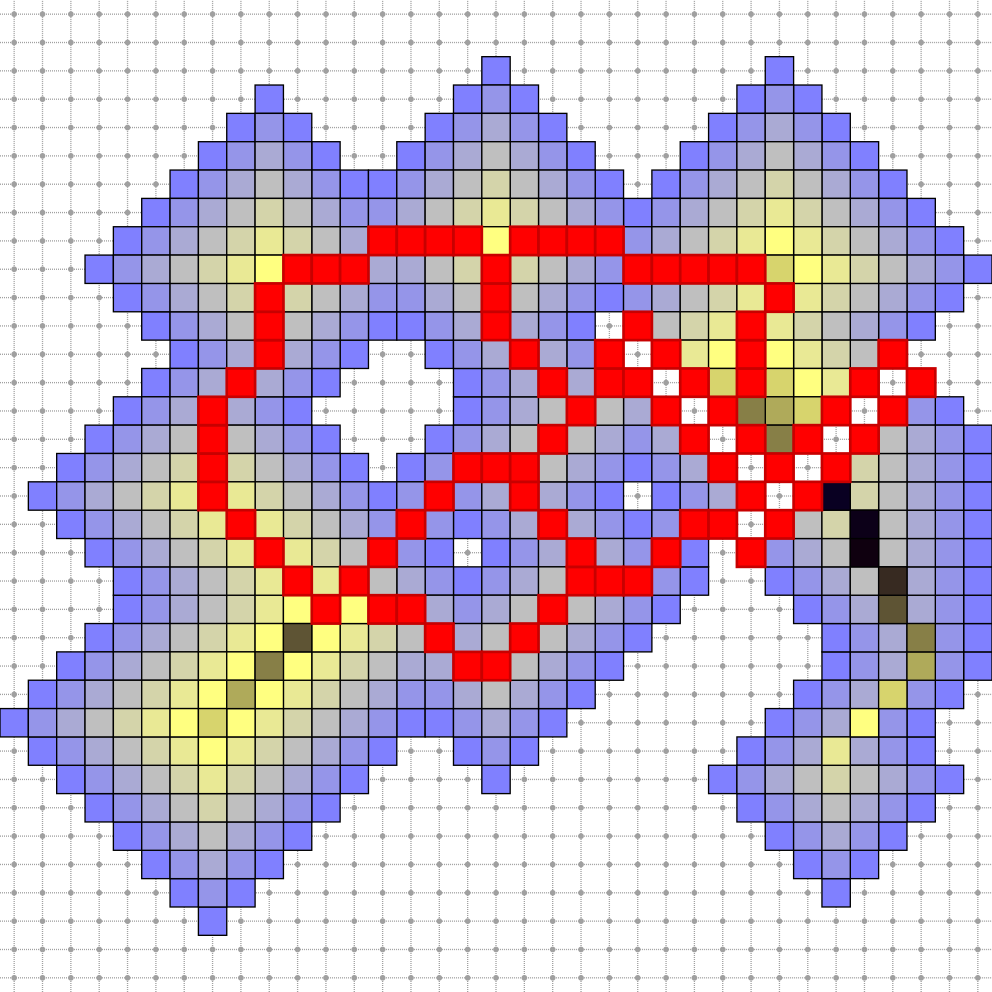
\includegraphics[width=0.4\textwidth]{shape-thinning-8-4} \\
%%       thinning in (4,8) &
%%       thinning in (8,4) \\
%%     \end{tabular}

%%     \texttt{tests/topology/testObject.cpp}
%%   \end{center}
%% \end{frame}
%% %------------------------------------------------------------------------------

%% %------------------------------------------------------------------------------
%% \begin{frame}
%%   \frametitle{Conclusion and perspectives}
  
%%   \begin{itemize}
%%   \item complete Rosenfeld's approach: curves and separation
%%   \item whole digital topology framework of Herman and Udupa
%%     \begin{itemize}
%%     \item digital surface as a couple of $\omega$-adjacent points
%%     \item immediate interior and exterior, interior and exterior
%%     \item $\kappa \lambda$-borders, $\kappa \lambda$-boundaries
%%     \item digital pictures
%%     \end{itemize}
%%   \item interpixel topology or cartesian cellular grid topology 
%%   \end{itemize}
%%   See on-line doc.: \Cb{Digital topology and digital objects}

%% \end{frame}
%% %------------------------------------------------------------------------------

\end{document}
